\chapter{Memory organization}

Larger memories are slower than smaller memories.
Fast memories are much more expensive than slow memories.

So instead of using a single large memory, modern systems use a hierarchy. 
Characterized by different technology, cost, dimensions and access mechanisms. The programmer sees an unique large memory space. The CPU sees a fast memory at acceptable cost.

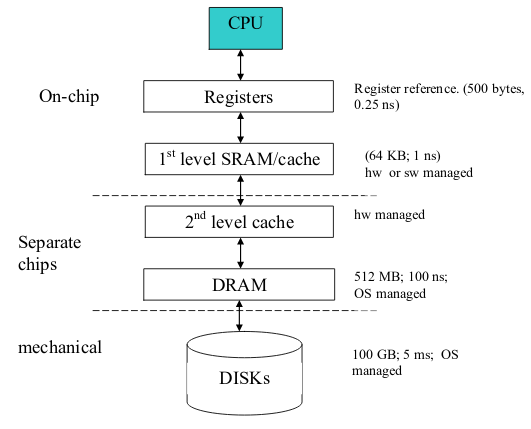
\includegraphics[width=.7\textwidth]{images/memory_hierarchy.png}
Hierarchies work well because memory access follows the principle of locality.

\paragraph{Locality}
\begin{itemize}
    \item \textbf{Temporal locality}:\\
    when a memory entry is referenced, with high probability it will be referenced again within a short time.
    
    \item \textbf{Spatial locality}:\\
    whenever a memory entry is referenced, with high probability reference will be made shortly to neighboring items.
\end{itemize}

\paragraph{Registers}
Registers are usually “exposed” to the programmer. Alternatively, the compiler allocates variables to registers.
Registers are usually placed into a regular register file. A register file consists of multiple read/write ports to allow parallel, simultaneous data accesses.
Typically, at least 2 read and 1 write ports are required to access operands of a single instruction.

Unfortunately, the size of the register file grows with the square of the number of ports so an excessive number of ports slows down the processors.

This quadratic increase in chip area is mostly due to the new additional input and output lines:\\
• Routing problems\\
• Internal bit cell loading increases -> larger power consumption\\
• Linear increment in delay with the number of ports

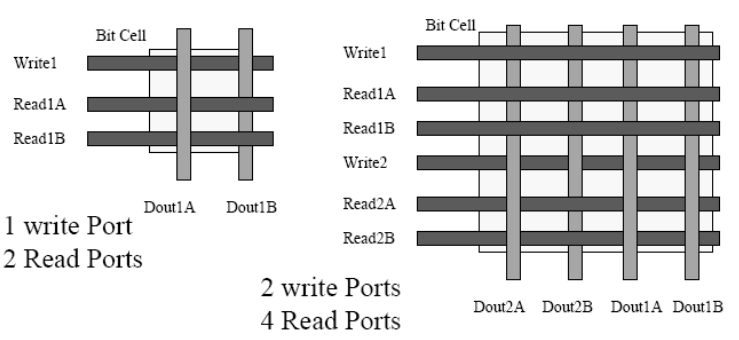
\includegraphics[width=.7\textwidth]{images/memory_bit_cells.png}

It is not profitable to have a register file with more than 15-20 ports: 12 is actually the best tradeoff when number of FU is larger than 4

\paragraph{The usual SRAM}
\begin{itemize}
    \item It is “exposed” to programmer and compiler
    \item Data transfers from/to memory are performed by \textbf{software}
    \item It is mostly used in low-end or specialized embedded processors where worst-case latency to recover data and power are the main issues
\end{itemize}

\paragraph{Cache}
\begin{itemize}
    \item Usually it is “transparent” to programmer and compiler
    \item Transfers from/to lower-level memories are performed by \textbf{hardware}
    \item It is mostly used in high-end processors where the power is less critical and average performance should be maximized
\end{itemize}

\paragraph{Scratch Pad}
It's a low power consumption solution.
The scratch pad is a buffer of memory (no cache) where most frequently used program functions instructions and data are allocated.
This approach requires a preliminary “profiling”to decide what instructions have to be placed into the scratch pad.
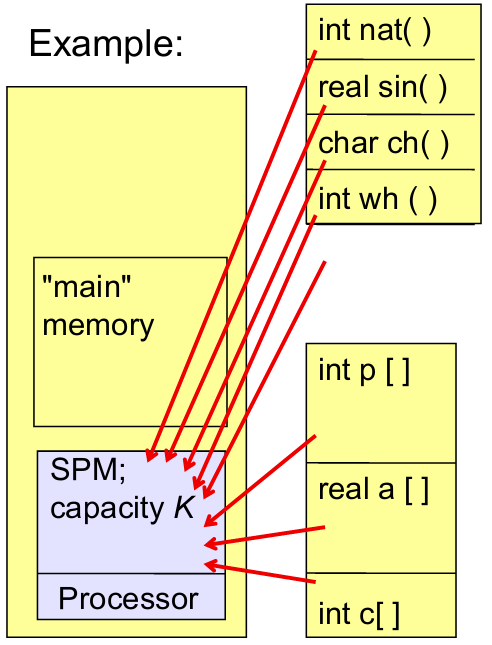
\includegraphics[width=.5\textwidth]{images/memory_scratch_pad.png}
Allocation usually performed statically at compile time (no HW support).
This kind of solution is very used in embedded systems because the program is usually fixed and it is a reasonable tradeoff between performance and power consumption.

\paragraph{Cache}
A cache is a special kind of memory based on SRAM cells which is used to store the data having the maximum probability to be used.
Cache can be either unified (i.e., simultaneously instruction-and data-cache) or split into I-cache and D-cache.

Definitions:
\begin{itemize}
    \item \textbf{Hit}: the item requested by the CPU is present in cache
    \item \textbf{Miss}: the item requested by the CPU is not present in cache
    \item \textbf{Hit rate}: fraction of memory accesses rewarded by hit
    \item \textbf{Miss rate}: fraction of memory accesses resulting in a miss (miss rate = 1 -hit rate)
    \item \textbf{Hit time}: access time (or clock cycles) to cache in the case of success (includes time to determine whether access is met by hit or miss)
    \item \textbf{Miss penalty}: time (or clock cycles) required to substitute a block of data in cache with another block from the lower-level storage
    \item \textbf{Miss time}: miss penalty + hit time, time required to obtain requested data in the case of miss
\end{itemize}

Cache performance is given in terms of average memory access time (AMAT)

$AMAT = hit-time + miss-rate * miss-penalty$\\

Cache performance affects CPU time

$CPU_{time} = IC * (CPI_{execution} + \frac{MEM_{accesses}}{IC} * miss-rate * miss-penalty) * T_{CLK}$

\paragraph{How cache works}
A cache is made of a number of \textbf{blocks} that contain \textbf{words} from memory.
The size of a block is a power of 2, to simplify addressing (e.g., a block is made of 32 words).
When a word is needed, its entire block is loaded from memory and placed somewhere in the cache.
Blocks that are next to each other in memory are not necessarily stored next to each other in the cache, and vice-versa.

The cache needs to store a block along with its actual address in memory.
The required address is compared to the address of all the blocks in the cache to find a match.
If found, it is a hit, otherwise it is a miss.

\paragraph{Problems in cache design}
\begin{itemize}
    \item \textbf{Placement problem}:\\
    Where to place a block transferred from lower to higher level
    \item \textbf{Search (or identification) problem}:\\
    how to determine whether the requested item is present or not
    \item \textbf{Substitution (or replacement) problem}:\\
    Which block present in the cache must be replaced by one in lower-level storage, in the case of a miss
    \item \textbf{Write strategy}:\\
    what happens when a write-to-memory instructions is executed?
\end{itemize}

\section{Direct-mapped cache}
Assume the cache is made of an array of $N_B$ blocks.
Let $B_{AR}$ be the address of the required block in RAM.

In a direct-mapped cache, the block can only be placed in the cache block at address $B_{AC}$:

$B_{AC} = B_{AR} mod N_B$

$B_{AC}$ is also called the index of the cache block.
If $N_B$ is a power of 2, then the index is equal to the $N_{AC} = log2(N_{B}$ least significant bits of $B_{AR}$.

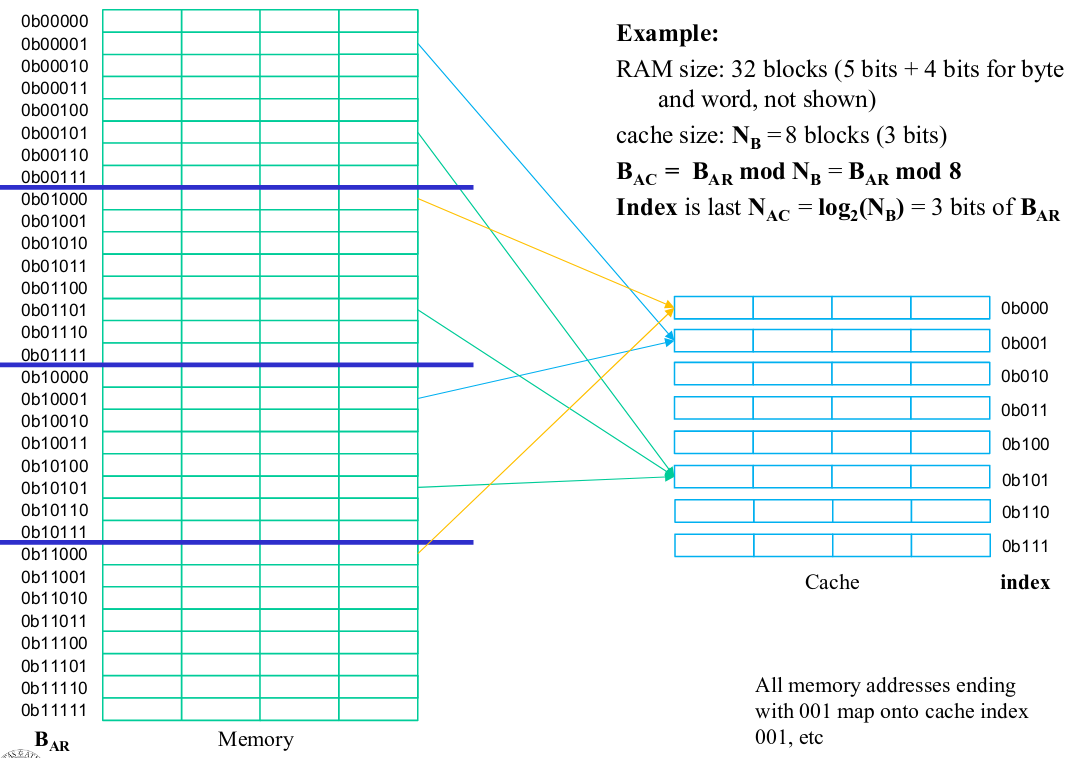
\includegraphics[width=\textwidth]{images/direct_mapped_cache.png}

\paragraph{Problems}
\begin{itemize}
    \item \textbf{Placement problem}:\\
    Trivial – the block from RAM can be mapped onto one cache block only
    \item \textbf{Search problem}:\\
    different memory blocks can be placed in the same cache block. How do we decide which location is mapped in the cache?\\
    \textbf{Solution}: each cache line must be provided with:
    \begin{itemize}
        \item A \textbf{tag field} containing the $N_{AR} - N_{AC}$ most significant bits of $B_{AR}$
        \item A \textbf{validity bit} - denotes whether block contains meaningful (valid) data.
    \end{itemize}
    \item \textbf{Replacement problem}:\\
    Trivial – the new block from RAM can be mapped onto one cache block only. Does not account for temporal locality! Block substituted may have been very recently used.
\end{itemize}

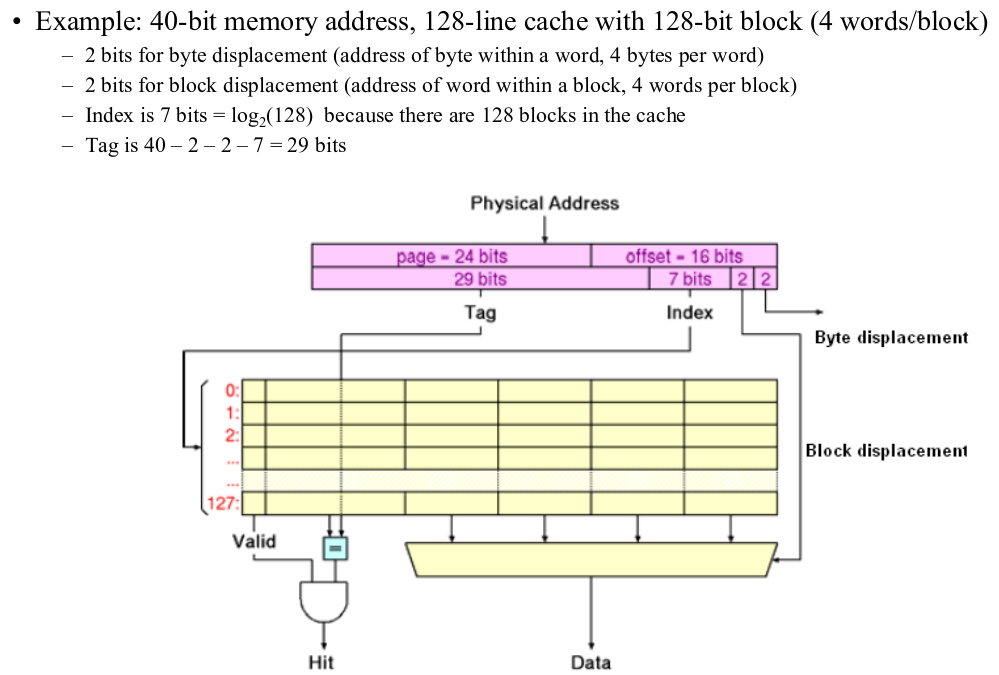
\includegraphics[width=\textwidth]{images/direct_mapped_cache_example.png}

\section{Fully associative cache}
In fully-associative cache every block of RAM can be mapped onto any block of cache (there is no constraint on Placement).
The search problem is tackled by running a parallel comparison of  the wanted address with all tags. So a large number of comparators is done and so it's very expensive in terms of area and power consumption.

The index is 0 bits and the tag is the complete address of the word minus the bits for block and byte displacements. 

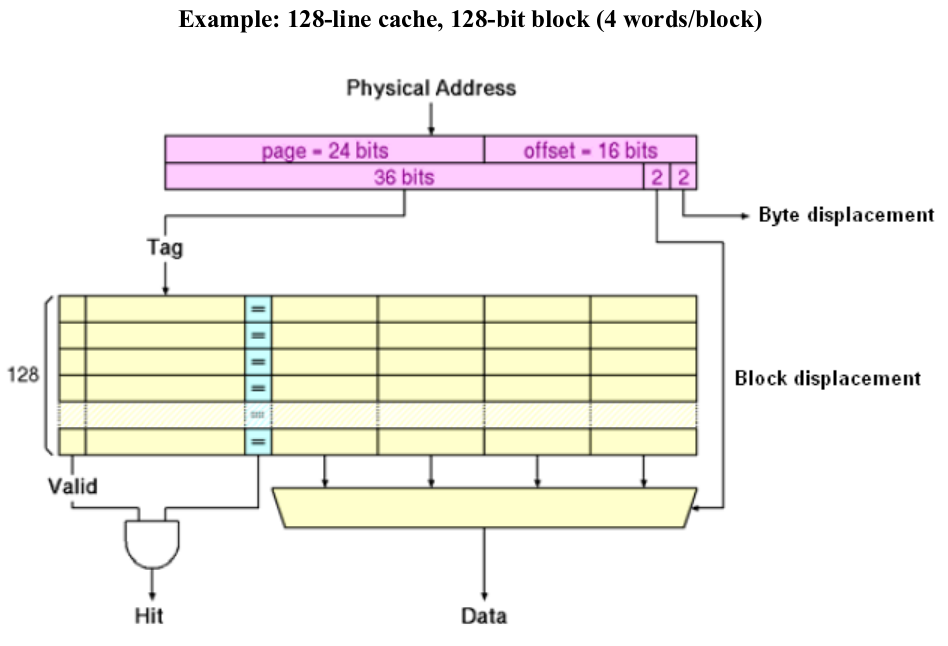
\includegraphics[width=\textwidth]{images/fully_associative_cache.png}

\paragraph{Replacement strategies}
\begin{itemize}
    \item \textbf{Random}:\\
    the block to be substituted is chosen randomly.
    \begin{itemize}
        \item \textit{pro}: It is simple. Minimum HW support (pseudo-random number generator)
        \item \textit{cons}: Efficiency in terms of miss rate is comparable to DM cache. In fact, temporal locality not taken into account.
    \end{itemize}
    \item \textbf{Least Recently Used (LRU)}:\\
    substitute the block left unused for the longest time.
    \begin{itemize}
        \item \textit{pro}: It fully exploits temporal locality. Maximum efficiency
        \item \textit{cons}: It requires HW support. The cost of this solution increases largely with the number of blocks. A counter per each block.
    \end{itemize}
    \item \textbf{First In First Out (FIFO)} (also called Round Robin) of length N:\\
    substitute the block used N accesses before the present one. Whether it was used during the last N-1accesses or not.
    \begin{itemize}
        \item \textit{pro}: This is the best tradeoff between performance and complexity. It is adopted in several recent systems.
        \item \textit{cons}: It just approximates the locality principle
    \end{itemize}
\end{itemize}

\section{N-way set-associative cache}
N-way set-associative cache is a tradeoff between DM and fully associative solutions.
Cache is arranged in $N_{set}$ sets ($N_{set}$ being a power of 2), each set including N blocks. Notice:  $N_{set} = N_B/ N$   where $N_B$ is the total number of blocks.

The index $I_{set}$ of the Set in cache corresponding to a given memory block address $B_{AR}$ is given by:\\
$I_{set} = B_{AR} mod N_{set}$

Each block within the set at index  $I_{set}$ can map onto any of the N cache blocks in the set, using fully associative technique.

The set in cache corresponding to block in RAM is identified as in DM cache (Index identifies Set). Within the set, block is identified with associative mechanisms (multiple tag comparisons in parallel).

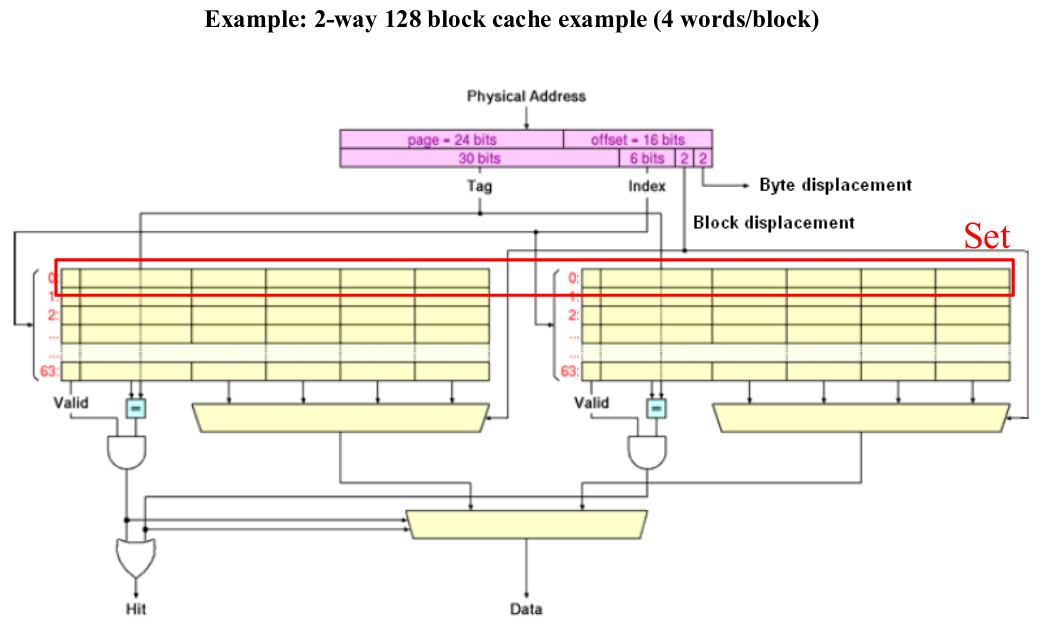
\includegraphics[width=\textwidth]{images/n-way_set_associative.png}

The direct mapped cache is a 1-way set associative cache (set = 1 block).
The fully associative cache has only one big set, the size of the whole cache.

\textbf{Advantages compared to fully associative cache}: comparators are fewer and smaller so cheaper and faster solutions.

\textbf{Advantages compared to direct-mapped cache}: better exploitation of temporal locality at a reasonable cost

The replacement of a block is performed by one of the techniques seen for associative cache (random, LRU or round-robin).

\section{Causes of cache miss}
\begin{itemize}
    \item \textbf{Compulsory misses}:\\
    at the time of the first access, a block is never present in cache. Not dependent on cache size and architecture (dependent on block size, though)
    \item \textbf{Capacity misses}:\\
    if the cache cannot contain all the blocks needed during execution of a program, capacity misses will occur due to blocks being discarded and later retrieved. This kind of misses decreases with cache size
    \item \textbf{Conflict misses}:\\
    in direct-mapped or set-associative caches, blocks that are replaced may have to be reloaded later in the same set – leading to collision (“conflict”) misses
\end{itemize}

\subsection{The write problem}
Write in caches are less frequent than reads.
Instruction fetch only requires memory reads.
“Load” instructions more frequent than “store”.

In Write to memory operations we ask:
\textbf{Speed}: implies writing to cache;
\textbf{Consistency}: information in lower-layer memories must always be consistent with information in cache.

\subsubsection{Write strategies:}
\paragraph{Write-through}
information is written \textbf{simultaneously} in cache block and in the main memory block. Consistency always respected, access time for writes is that of the lower level of memory, so lower performance.

\paragraph{Write-back}

